\chapter{Construção}
\label{chap:Construcao}

Para construção do \emph{software} aplicativo foi utilizado uma arquitetura em
três camadas: sensor, distribuidor de acesso (\emph{IoT gateway}) e apresentação
(\emph{Web}). Nesta divisão os sensores capturam as informações dos dispositivos
e repassam para a camada seguinte, no \emph{gateway} todas as partes se
encontram para fornecer e solicitar informações e, por último a camada de
apresentação coleta o que é enviado dos sensores e gera uma página \emph{Web}
para visualização dos dados capturados.

Esta divisão está de acordo com o padrão encontrado em outras aplicações
\emph{IoT} onde a última camada usualmente varia entre apresentação e mineração
de dados (\emph{Data Mining}).

A camada de sensor utilizou as tecnologias \emph{Node.js}, \emph{TShark} parte
do \emph{Wireshark} e \emph{MQTT.js}. A camada \emph{gateway} foi composta
basicamente pelo \emph{MQTT Broker} \emph{Mosquitto}. Por fim a camada de
apresentação utlizou as tecnologias \emph{Node.js}, \emph{MQTT.js}, \emph{html},
\emph{css}, \emph{javascript}, \emph{Bootstrap} e \emph{Google Maps API}.

\begin{figure}[htb]
	\caption{\label{fig-arq-app}Arquitetura da aplicação}
	\begin{center}
		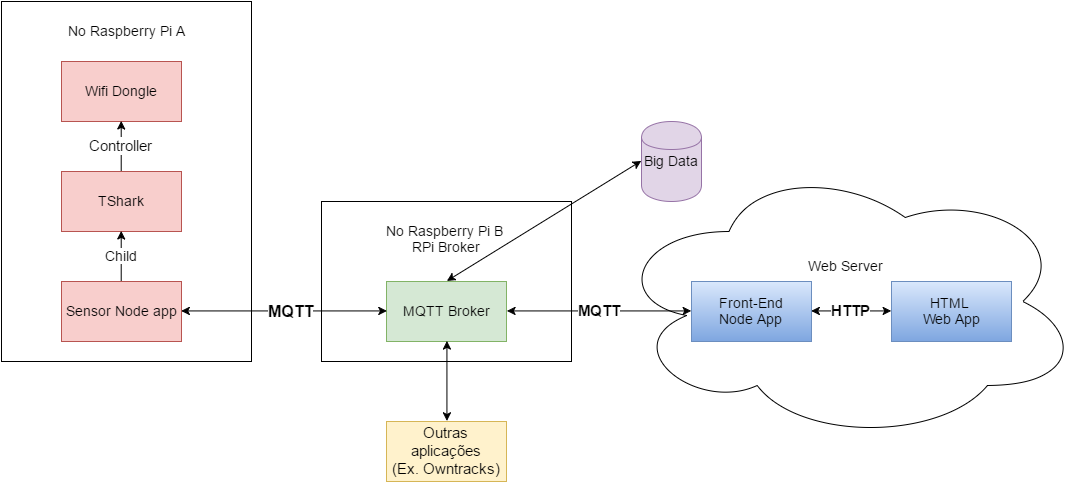
\includegraphics[width=1\textwidth]{050-construcao/esquema-proj.png}
	\end{center}
	\legend{Fonte: Elaborada pelo autor}
\end{figure}


\section{Sensor}
\label{sec:app-sensor}


A aplicação sensor tem como objetivo capturar, avaliar e classificar pacotes de
Wi-Fi, inferir estatísticas de dispositivos e fornecer estas informações para
os interessados através do \emph{gateway}.

Para fazer a caputra dos pacotes na aplicação final, diferente do que foi
demonstrado na \autoref{subsec:testes-rpi}, em especial o \emph{airodump-ng} e
sua interface demonstrada na \autoref{fig-airodump}, foi utilizado o programa
\emph{TShark} cujo modo de operação serve melhor para a construção dos
\emph{Streams} que serão abodados em breve.

\begin{citacao}

	TShark é uma versão orientada ao terminal do Wireshark projetada para capturar
	e exibir pacotes quando uma interface de usuário interativa não é necessária ou
	disponível. Ele suporta as mesmas opções como wireshark. \

	\citeonline{tshark} Tradução Nossa.
\end{citacao}

Como foi estabelecido no capítulo anterior, \emph{TShark}  utiliza a saída
padrão  do terminal (\emph{stdout}) como sua saída principal, esta
característica foi explorada com aplicação \emph{nodejs}. Mais especificamente
com módulo \emph{child\_process},  que provê uma API que permite a criação e
controle de processos filhos do processo \emph{nodejs}.

\begin{citacao}

	Node.js é uma estrutura em tempo de execução construida sobre o motor de
	execução JavaScript V8 do Chrome. Node.js utiliza um modelo orientado a
	evento, de entrada e saída não bloqueante que o faz leve e eficiente.
	O ecosistema de pacotes do Node.js, npm, é o maior ecosistema de bibliotecas
	de código livre no mundo. \

	\citeonline{nodejs} Tradução Nossa.
\end{citacao}

Como também foi estabelecido anterioremte o \emph{TShark} é executado com o
comando e argumentos como mostrado à seguir, a diferença em relação aos testes e
na escolha da plataforma é a forma de execução, na maneira mostrada o processo é
criado utilizando o módulo \emph{child\_process} \cite{child_process} e os
argumentos são passados como um vetor (\emph{Array}).

\begin{lstlisting}[language=java]
const spawn = require('child_process').spawn;
const tsharkProcessoFilho = spawn(
	'tshark', [
		'-I',
		'-i', childIface,
		'-T', 'fields',
		'-E', 'separator=,',
		'-E', 'quote=d',
		'-e', 'wlan.sa',
		'-e', 'wlan.sa_resolved',
		'-e', 'wlan.ta',
		'-e', 'wlan.ta_resolved',
		'-e', 'radiotap.dbm_antsignal',
		'-e', 'wlan_mgt.ssid',
		'-Y', 'wlan.sa'
	]);
\end{lstlisting}

Para utilizar o resultado gerado pelo \emph{TShark} utilizamos outro método do
módulo \emph{child\_process} juntamente com a estrutura de \emph{Stream}
\cite{stream} que provê o método \emph{pipe(destination[, options])} que permite,
de maneira análoga ao operador '|' no terminal também chamado de \emph{pipe},
redirecionar a saída de um processo ou \emph{stream} de leitura para outro
processo ou \emph{stream} de escrita.

Com isso nos falta apenas um \emph{stream} de escrita que receba a saída do
\emph{TShark} que foi definida no formato CSV. Para isso biblioteca extra
\emph{fast-csv} deve ser instalada. Com ela podemos criar o \emph{stream}
necessário e configura-lo interpretar os resultados \cite{fast-csv}.

\begin{lstlisting}[language=java]
const csv = require("fast-csv");
let csvStream = csv()
  .on("data", function(data){
    let wlan = {
      sa            : data[0], // sender address
      sa_resolved   : data[1], // sender address resolved
      ta            : data[2], // transmitter address
      ta_resolved   : data[3], // transmitter address resolved
    };
    let radiotap = {
      dbm_antsignal : data[4], // potencia de sinal (rss)
    };
    let wlan_mgt = {
      ssid          : data[5], // nome da rede no pacote Beacon
    };
    let packet = {
      wlan     : wlan,
      radiotap : radiotap,
      wlan_mgt : wlan_mgt,
    };
    processarPacote(packet);
  })
  .on("end", function(){
    console.log("done with tshark");
  });

tsharkProcessoFilho.stdout.setEncoding('utf8');
tsharkProcessoFilho.stdout.pipe(csvStream);
\end{lstlisting}

Nesta ultima linha pode-se observar a operação de redirecionamento (\emph{pipe})
de \emph{stream} da saída padrão do processo filho (\emph{stdout}) para o
\emph{stream} de escrita descrito e configurado com o \emph{fast-csv}. A parte
faltante é o processamento dos pacotes e envio das inferências do sensor para o
\emph{gateway}.

// inferencias

// mqtt

\section{Gateway}
\label{sec:app-gw}

\begin{citacao}

	Eclipse Mosquitto™ is an open source (EPL/EDL licensed) message broker that
	implements the MQTT protocol versions 3.1 and 3.1.1. MQTT provides a lightweight
	method of carrying out messaging using a publish/subscribe model. This makes it
	suitable for "Internet of Things" messaging such as with low power sensors or
	mobile devices such as phones, embedded computers or microcontrollers like the
	Arduino. \

	\citeonline{nodejs} Tradução Nossa.
\end{citacao}


\section{Apresentação Web}
\label{sec:app-web}


\begin{figure}[htb]
	\caption{\label{fig-web-app}Web APP}
	\begin{center}
		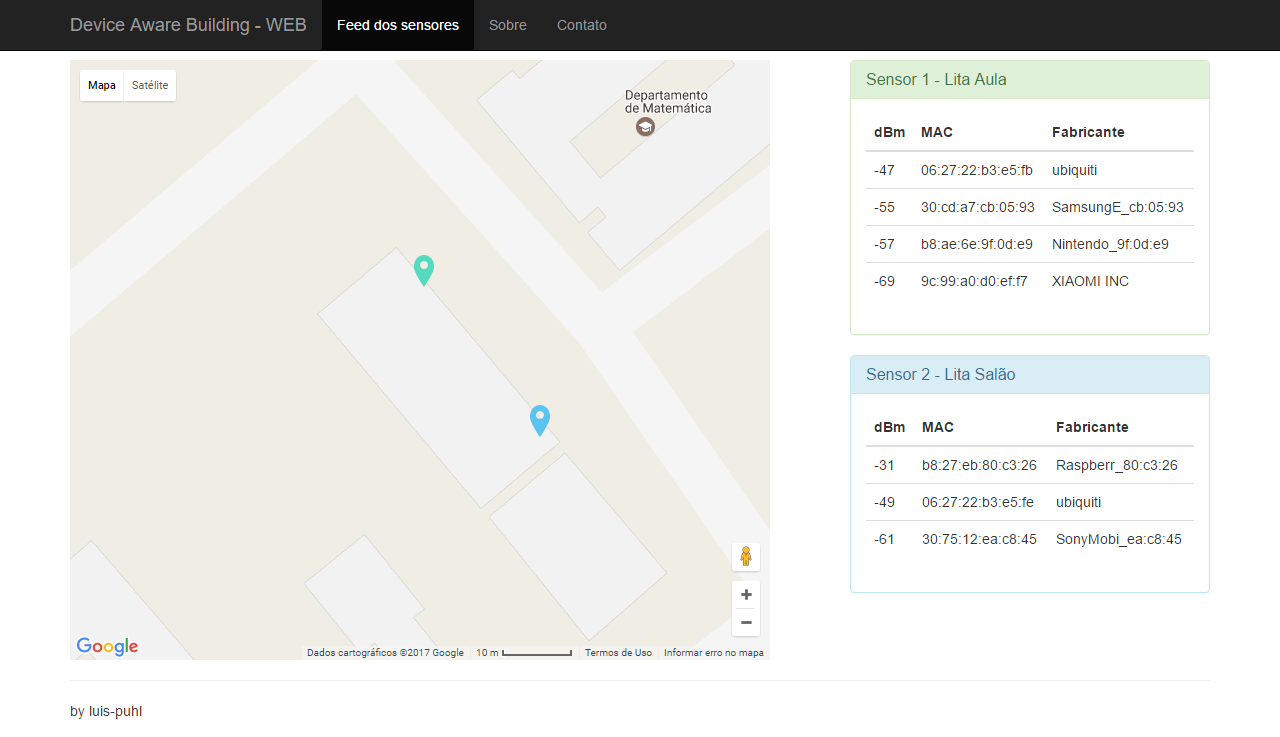
\includegraphics[width=1\textwidth]{050-construcao/web-app.png}
	\end{center}
	\legend{Fonte: Elaborada pelo autor}
\end{figure}
